%%%%%%%%%%%%%%%%%%%%%%%%%%%%%%%%%%%%%%%%%
% Beamer Presentation
% LaTeX Template
% Version 1.0 (10/11/12)
%
% This template has been downloaded from:
% http://www.LaTeXTemplates.com
%
% License:
% CC BY-NC-SA 3.0 (http://creativecommons.org/licenses/by-nc-sa/3.0/)
%
%%%%%%%%%%%%%%%%%%%%%%%%%%%%%%%%%%%%%%%%%

%----------------------------------------------------------------------------------------
%	PACKAGES AND THEMES
%----------------------------------------------------------------------------------------

\documentclass{beamer}

\mode<presentation> {

% The Beamer class comes with a number of default slide themes
% which change the colors and layouts of slides. Below this is a list
% of all the themes, uncomment each in turn to see what they look like.

%\usetheme{default}
%\usetheme{AnnArbor}
%\usetheme{Antibes}
%\usetheme{Bergen}
%\usetheme{Berkeley}
%\usetheme{Berlin}
%\usetheme{Boadilla}
%\usetheme{CambridgeUS}
%\usetheme{Copenhagen}
%\usetheme{Darmstadt}
%\usetheme{Dresden}
%\usetheme{Frankfurt}
%\usetheme{Goettingen}
%\usetheme{Hannover}
%\usetheme{Ilmenau}
%\usetheme{JuanLesPins}
%\usetheme{Luebeck}
%\usetheme{Madrid}
%\usetheme{Malmoe}
%\usetheme{Marburg}
%\usetheme{Montpellier}
%\usetheme{PaloAlto}
%\usetheme{Pittsburgh}
%\usetheme{Rochester}
%\usetheme{Singapore}
%\usetheme{Szeged}
\usetheme{Warsaw}

% As well as themes, the Beamer class has a number of color themes
% for any slide theme. Uncomment each of these in turn to see how it
% changes the colors of your current slide theme.

%\usecolortheme{albatross}
%\usecolortheme{beaver}
%\usecolortheme{beetle}
%\usecolortheme{crane}
%\usecolortheme{dolphin}
%\usecolortheme{dove}
%\usecolortheme{fly}
%\usecolortheme{lily}
%\usecolortheme{orchid}
%\usecolortheme{rose}
%\usecolortheme{seagull}
\usecolortheme{seahorse}
%\usecolortheme{whale}
%\usecolortheme{wolverine}

%\setbeamertemplate{footline} % To remove the footer line in all slides uncomment this line
%\setbeamertemplate{footline}[page number] % To replace the footer line in all slides with a simple slide count uncomment this line

%\setbeamertemplate{navigation symbols}{} % To remove the navigation symbols from the bottom of all slides uncomment this line
}

\usepackage{graphicx}
\usepackage{overpic}
\usepackage{booktabs}
\documentclass[11pt]{article}
\usepackage[BoldFont,SlantFont,CJKsetspaces,CJKchecksingle]{xeCJK}
\setCJKmainfont[BoldFont=SimHei]{SimSun}
\setCJKmonofont{SimSun}% 设置缺省中文字体

%----------------------------------------------------------------------------------------
%	TITLE PAGE
%----------------------------------------------------------------------------------------

\title[考核报告]{$\eta_c\to K_S^0 K \pi$分支比的测量}

\author{马旭宁\inst{1} \and 王至勇\inst{2} \and 喻纯旭\inst{1}}
\institute[]{\inst{1} 南开大学 \and \inst{2} 高能所}

\date{\today}

\begin{document}

\begin{frame}
\titlepage
\end{frame}

%\begin{frame}
%\tableofcontents
%\end{frame}

\section{Motivation}
\begin{frame}{Motivation}
\begin{itemize}
\item 为了测量辐射跃迁相关分支比,需要$\eta_c \to K_S^0 K \pi$的精确分支比\\
\item 之前对 $\eta_c \to K_S^0 K \pi$分支比的测量精度不够高\\
\end{itemize}
\end{frame}

\section{进度}
\subsection{之前的工作}
\subsubsection{导言}
\begin{frame}{导言}
通过衰变道
\begin{center}
$\psi\prime\to\pi^0h_c$\\
$h_c\to\gamma\eta_c$\\
$\eta_c \to K_S^0 K \pi$\\
\end{center}
来测量\\
\begin{center}
$\eta_c \to K_S^0 K \pi$,\\
\end{center}
的分支比
\bigskip
基本思路
        \begin{center}
$Br(\eta_c\to K^0_S K \pi) = 
\frac{ N^{exc}_{sig} }{ N^{inc}_{sig} } 
\times \frac{ \epsilon^{inc} }{ \epsilon^{exc} }
\times \frac{ 1 }{ Br(K^0_S\to\pi^+\pi^-) }
$
\end{center}
\end{frame}

\subsubsection{结果}
\begin{frame}{结果}
\begin{columns}[c]
\begin{column}{0.7\textwidth}
遍举过程结果:\\
    \begin{columns}[c]
    \begin{column}{0.45\textwidth}
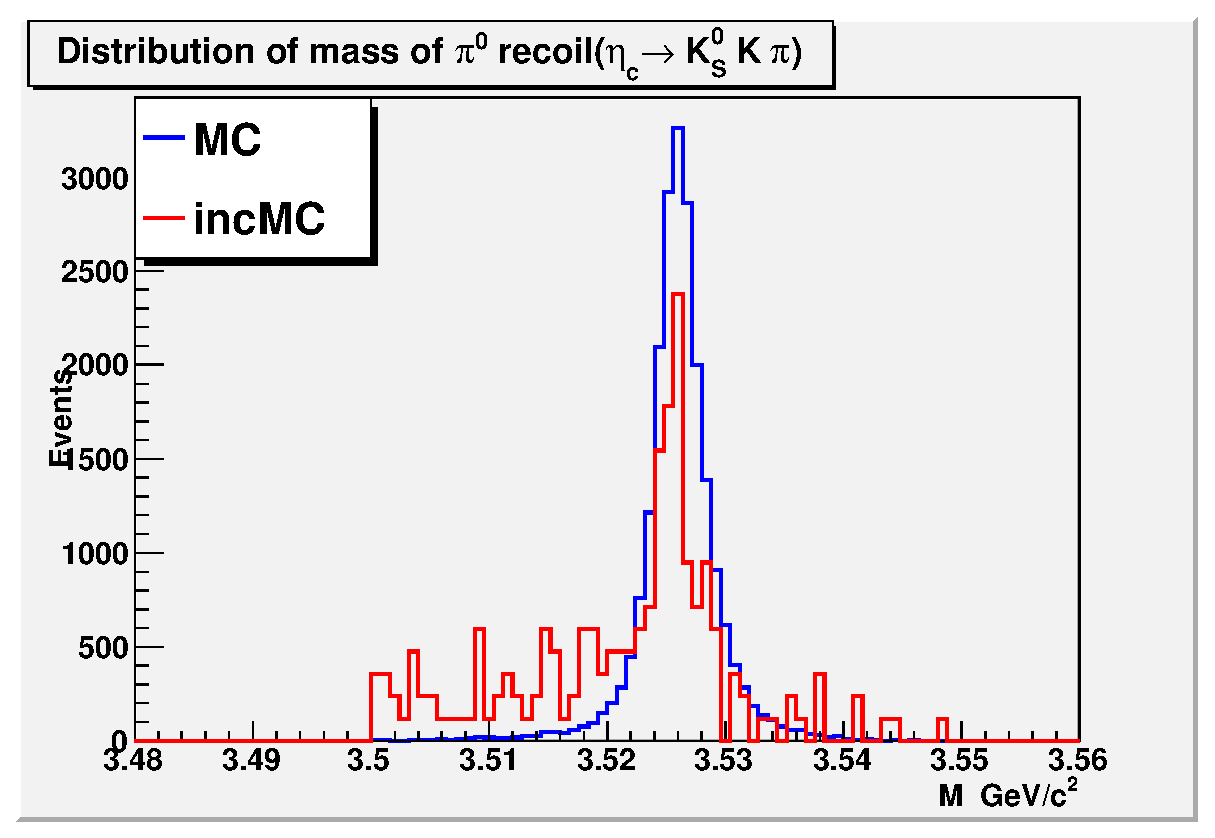
\includegraphics[width=0.85\textwidth,angle=0]{figures/kskp_results/Pi0hc_invariant_mass_of_hc.eps}\\
        \end{column}
    \begin{column}{0.45\textwidth}
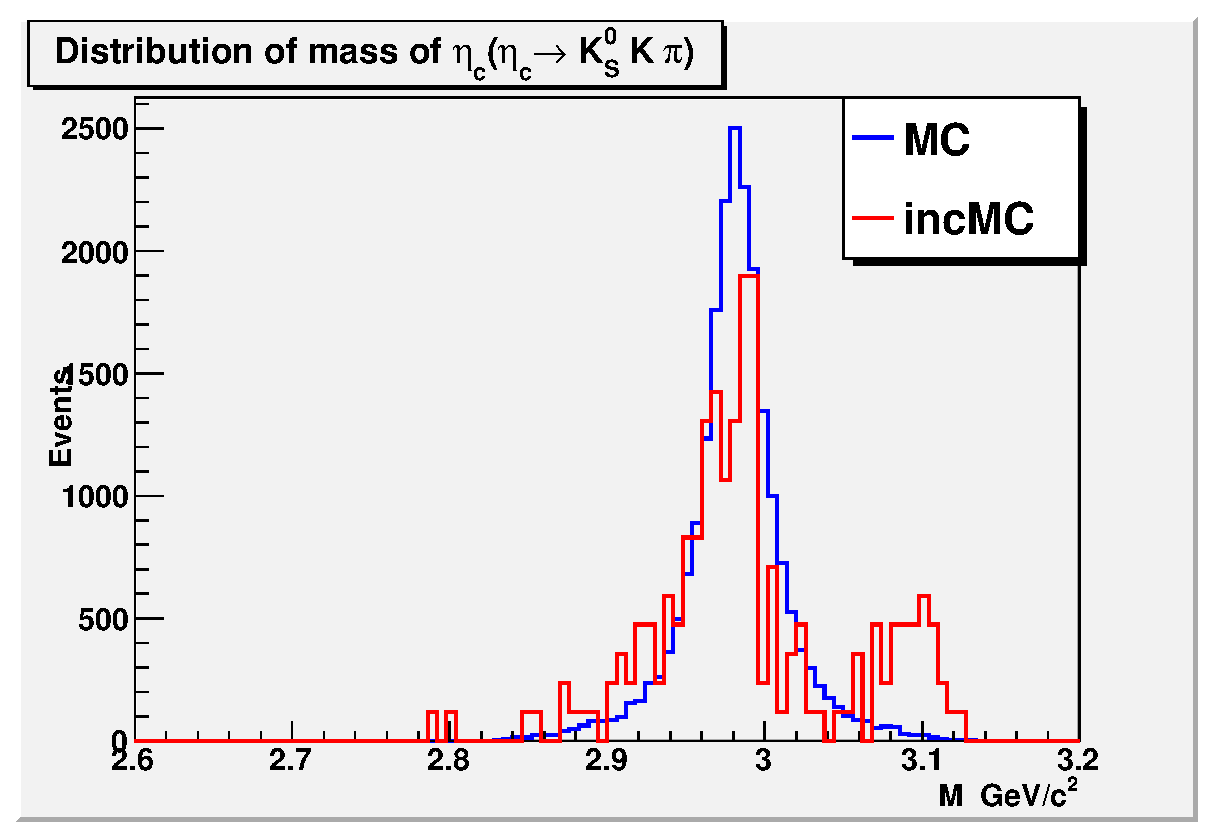
\includegraphics[width=0.85\textwidth,angle=0]{figures/kskp_results/Pi0hc_invariant_mass_of_etac.eps}\\
        \end{column}
        \end{columns}
        \vskip -0.5cm
\begin{table}[htbp]
\begin{center}
\begin{tiny}
\begin{tabular}{c|c|c}\hline\hline
选择条件& 剩余事例数& 效率(\%) \\
        \hline
None & 200K &  100 \\
$N_{GoodL}\le20$ \&\&$N_{charge}=0$ & 104709 & 52.35\\
$3\le N_{\gamma}\le100$ &75919 & 37.96 \\
$N(E_{\gamma_{E1}}\in(0.3,0.7))\ge 1$ & 64.02 & 24.30 \\
$N_{\gamma\pi^0 list}\ge 1$ & 43773 & 21.89 \\
$2\le N_{Good}\le 4,N_{GoodL}\ge 4,N_{\gamma}\ge 3,N_{\pi^0}\ge 1$ & 38043 & 19.02 \\
$\chi^2\le 1000$ & 27927 & 13.96 \\
$3.5<M^{recoil}_{\pi^0}<3.55 GeV$ & 26721  & 13.36\\
$\chi^2_{4C}\le 55$ & 23314 & 11.66\\
$0.4<E_{\gamma_{E1}}<0.6 GeV $ &22617  & 11.30 \\
$|m^{recoil}_{\pi^0 \pi^0}-M_{J/\psi}|<0.03$ & 22553  & 11.28 \\
$|m^{recoil}_{\gamma}-M_{\chi_{c0}}|<0.027$ & 21403 & 10.70 \\
$|m^{recoil}_{\gamma}-M_{\chi_{c1}}|<0.028$ &21263  & 10.63\\
$|m^{recoil}_{\gamma}-M_{\chi_{c2}}|<0.001$ &21184  & 10.59\\
$|m^{recoil}_{\pi^+ \pi^-}-M_{J/\psi}|<0.004$ & 21131  & 10.57\\
\hline
\hline
\end{tabular}
\end{tiny}
\end{center}
\end{table}
\end{column}
\begin{column}{0.3\textwidth}
单举过程结果:\\
\bigskip
\begin{overpic}[width=0.95\textwidth,angle=0]{figures/Pi0_recoil.eps}
\put(0,0){\tiny\color{brown}{$\pi^0$ 反冲质量分布}}
\end{overpic}
\bigskip
\bigskip
\bigskip
\begin{overpic}[width=0.95\textwidth,angle=0]{figures/SignalAndBackground.eps}
\put(0,0){\tiny\color{brown}{$\pi^0$ $\gamma$反冲质量分布}}
\end{overpic}
\end{column}
\end{columns}
\end{frame}

\subsection{当前的工作}

\subsubsection{导言}
\begin{frame}{导言}
为了进一步提高精度,我们开始研究$XYZ$数据,目前选了四个能量点$4230$, $4260$, $4360$, $4420$.\\
我们研究的衰变道为:
\begin{center}
$e^+e^-\to\pi^+\pi^-h_c$\\
$h_c\to\gamma\eta_c$\\
$\eta_c \to K_S^0 K \pi$\\
\end{center}
\bigskip
思路跟$\psi\prime$分析一样。\\
\end{frame}

\subsubsection{结果}
\begin{frame}{遍举过程结果}
\vskip -0.2cm
\begin{columns}[c]
\begin{column}{0.5\textwidth}
\begin{overpic}[width=0.94\textwidth]{figures/Exclusive/PipihcExclusive_4230_data_with_optimization.eps}
\put(14,52){\scriptsize\color{blue}{\bf $\sqrt{s} = 4.23GeV$}}
\put(14,42){\scriptsize\color{blue}{\bf $\chi^2<65$}}
\end{overpic}
\vskip 0.2 cm
\begin{overpic}[width=0.94\textwidth]{figures/Exclusive/PipihcExclusive_4360_data_with_optimization.eps}
\put(14,52){\scriptsize\color{blue}{\bf $\sqrt{s} = 4.36GeV$}}
\put(14,42){\scriptsize\color{blue}{\bf $\chi^2<50$}}
\end{overpic}
\end{column}
\begin{column}{0.5\textwidth}
\begin{overpic}[width=0.94\textwidth]{figures/Exclusive/PipihcExclusive_4260_data_with_optimization.eps}
\put(14,52) {\scriptsize\color{blue}{\bf $\sqrt{s} = 4.26GeV$}}
\put(14,42){\scriptsize\color{blue}{\bf $\chi^2<25$}}
\end{overpic}
\vskip 0.2 cm
\begin{overpic}[width=0.94\textwidth]{figures/Exclusive/PipihcExclusive_4420_data_with_optimization.eps}
\put(14,52) {\scriptsize\color{blue}{\bf $\sqrt{s} = 4.42GeV$}}
\put(14,42){\scriptsize\color{blue}{\bf $\chi^2<30$}}
\end{overpic}
\end{column}
\end{columns}
\end{frame}

\begin{frame}
\frametitle{单举过程结果}
我们使用了sideband的方法来研究单举过程
\vskip -0.5cm
\begin{columns}[c]
\begin{column}{0.5\textwidth}
\begin{overpic}[width=1.0\textwidth]{figures/Inclusive/PipihcInclusive_4260_data_recoil_pipi_without_cut.eps}
\put(23,10){\tiny\color{red}{\bf$3.485$}}
\put(33,10){\tiny\color{red}{\bf$3.505$}}
\put(34,13){\tiny\color{green}{\bf$3.515$}}
\put(43,13){\tiny\color{green}{\bf$3.535$}}
\put(45,10){\tiny\color{red}{\bf$3.545$}}
\put(55,10){\tiny\color{red}{\bf$3.565$}}
\end{overpic}
\end{column}
\begin{column}{0.5\textwidth}
\begin{columns}[c]
\begin{column}{0.5\textwidth}
\begin{overpic}[width=1.0\textwidth]{figures/Inclusive/PipihcInclusive_4230_data_sideband_2.eps}
\put(10,50) {\scriptsize\color{blue}{\bf $\sqrt{s} = 4.23GeV$}}
\end{overpic}
\begin{overpic}[width=1.0\textwidth]{figures/Inclusive/PipihcInclusive_4260_data_sideband_2.eps}
\put(10,50) {\scriptsize\color{blue}{\bf $\sqrt{s} = 4.26GeV$}}
\end{overpic}
\end{column}
\begin{column}{0.5\textwidth}
\begin{overpic}[width=1.0\textwidth]{figures/Inclusive/PipihcInclusive_4360_data_sideband_2.eps}
\put(10,50) {\scriptsize\color{blue}{\bf $\sqrt{s} = 4.36GeV$}}
\end{overpic}
\begin{overpic}[width=1.0\textwidth]{figures/Inclusive/PipihcInclusive_4420_data_sideband_2.eps}
\put(10,50) {\scriptsize\color{blue}{\bf $\sqrt{s} = 4.42GeV$}}
\end{overpic}
\end{column}
\end{columns}
\end{column}
\end{columns}
\end{frame}

\subsubsection{同时拟合}
\begin{frame}{初步拟合}
\begin{columns}[c]

\begin{column}{0.5\textwidth}
\begin{overpic}[width=0.94\textwidth]{figures/pics/Pipihc_4230_data_fit_simultaneous.eps}
\put(10,50) {\tiny\color{blue}{\bf $\sqrt{s} = 4.23GeV$}}
\end{overpic}
\begin{overpic}[width=0.94\textwidth]{figures/pics/Pipihc_4360_data_fit_simultaneous.eps}
\put(10,50) {\tiny\color{blue}{\bf $\sqrt{s} = 4.36GeV$}}
\end{overpic}
\end{column}

\begin{column}{0.5\textwidth}
\begin{overpic}[width=0.94\textwidth]{figures/pics/Pipihc_4260_data_fit_simultaneous.eps}
\put(10,50) {\tiny\color{blue}{\bf $\sqrt{s} = 4.26GeV$}}
\end{overpic}
\begin{overpic}[width=0.94\textwidth]{figures/pics/Pipihc_4420_data_fit_simultaneous.eps}
\put(10,50) {\tiny\color{blue}{\bf $\sqrt{s} = 4.42GeV$}}
\end{overpic}
\end{column}
\end{columns}
\end{frame}

\section{当前遇到的问题}
\subsection{拟合}
\begin{frame}{效率曲线和分辨曲线}
\vskip -0.2cm
\begin{columns}[c]

\begin{column}{0.25\textwidth}
\begin{overpic}[width=0.94\textwidth]{figures/Fit/Pipihc_Exclusive_4230_efficiency_curve.eps}
\put(16,22){\tiny\color{blue}{\bf $\sqrt{s} = 4.23GeV$}}
\put(14,12){\tiny\color{blue}{\bf Exclusive}}
\end{overpic}
\begin{overpic}[width=0.94\textwidth]{figures/Fit/Pipihc_Exclusive_4360_efficiency_curve.eps}
\put(16,22){\tiny\color{blue}{\bf $\sqrt{s} = 4.36GeV$}}
\put(14,12){\tiny\color{blue}{\bf Exclusive}}
\end{overpic}
\begin{overpic}[width=0.94\textwidth]{figures/Fit/Pipihc_Exclusive_4230_resolution_curve.eps}
\put(16,22){\tiny\color{blue}{\bf $\sqrt{s} = 4.23GeV$}}
\put(14,12){\tiny\color{blue}{\bf Exclusive}}
\end{overpic}
\begin{overpic}[width=0.94\textwidth]{figures/Fit/Pipihc_Exclusive_4360_resolution_curve.eps}
\put(16,22){\tiny\color{blue}{\bf $\sqrt{s} = 4.36GeV$}}
\put(14,12){\tiny\color{blue}{\bf Exclusive}}
\end{overpic}
\end{column}

\begin{column}{0.25\textwidth}
\begin{overpic}[width=0.94\textwidth]{figures/Fit/Pipihc_Exclusive_4260_efficiency_curve.eps}
\put(16,22){\tiny\color{blue}{\bf $\sqrt{s} = 4.26GeV$}}
\put(14,12){\tiny\color{blue}{\bf Exclusive}}
\end{overpic}
\begin{overpic}[width=0.94\textwidth]{figures/Fit/Pipihc_Exclusive_4420_efficiency_curve.eps}
\put(16,22){\tiny\color{blue}{\bf $\sqrt{s} = 4.42GeV$}}
\put(14,12){\tiny\color{blue}{\bf Exclusive}}
\end{overpic}
\begin{overpic}[width=0.94\textwidth]{figures/Fit/Pipihc_Exclusive_4260_resolution_curve.eps}
\put(16,22){\tiny\color{blue}{\bf $\sqrt{s} = 4.26GeV$}}
\put(14,12){\tiny\color{blue}{\bf Exclusive}}
\end{overpic}
\begin{overpic}[width=0.94\textwidth]{figures/Fit/Pipihc_Exclusive_4420_resolution_curve.eps}
\put(16,22){\tiny\color{blue}{\bf $\sqrt{s} = 4.42GeV$}}
\put(14,12){\tiny\color{blue}{\bf Exclusive}}
\end{overpic}
\end{column}

\begin{column}{0.25\textwidth}
\begin{overpic}[width=0.94\textwidth]{figures/Fit/Pipihc_Inclusive_4230_efficiency_curve.eps}
\put(16,22){\tiny\color{blue}{\bf $\sqrt{s} = 4.23GeV$}}
\put(14,12){\tiny\color{blue}{\bf Inclusive}}
\end{overpic}
\begin{overpic}[width=0.94\textwidth]{figures/Fit/Pipihc_Inclusive_4360_efficiency_curve.eps}
\put(16,22){\tiny\color{blue}{\bf $\sqrt{s} = 4.36GeV$}}
\put(14,12){\tiny\color{blue}{\bf Inclusive}}
\end{overpic}
\begin{overpic}[width=0.94\textwidth]{figures/Fit/Pipihc_Inclusive_4230_resolution_curve.eps}
\put(16,22){\tiny\color{blue}{\bf $\sqrt{s} = 4.23GeV$}}
\put(14,12){\tiny\color{blue}{\bf Inclusive}}
\end{overpic}
\begin{overpic}[width=0.94\textwidth]{figures/Fit/Pipihc_Inclusive_4360_resolution_curve.eps}
\put(16,22){\tiny\color{blue}{\bf $\sqrt{s} = 4.36GeV$}}
\put(14,12){\tiny\color{blue}{\bf Inclusive}}
\end{overpic}
\end{column}

\begin{column}{0.25\textwidth}
\begin{overpic}[width=0.94\textwidth]{figures/Fit/Pipihc_Inclusive_4260_efficiency_curve.eps}
\put(16,22){\tiny\color{blue}{\bf $\sqrt{s} = 4.26GeV$}}
\put(14,12){\tiny\color{blue}{\bf Inclusive}}
\end{overpic}
\begin{overpic}[width=0.94\textwidth]{figures/Fit/Pipihc_Inclusive_4420_efficiency_curve.eps}
\put(16,22){\tiny\color{blue}{\bf $\sqrt{s} = 4.42GeV$}}
\put(14,12){\tiny\color{blue}{\bf Inclusive}}
\end{overpic}
\begin{overpic}[width=0.94\textwidth]{figures/Fit/Pipihc_Inclusive_4260_resolution_curve.eps}
\put(16,22){\tiny\color{blue}{\bf $\sqrt{s} = 4.26GeV$}}
\put(14,12){\tiny\color{blue}{\bf Inclusive}}
\end{overpic}
\begin{overpic}[width=0.94\textwidth]{figures/Fit/Pipihc_Inclusive_4420_resolution_curve.eps}
\put(16,22){\tiny\color{blue}{\bf $\sqrt{s} = 4.42GeV$}}
\put(14,12){\tiny\color{blue}{\bf Inclusive}}
\end{overpic}
\end{column}

\end{columns}
\end{frame}

\section{总结}
\begin{frame}{总结}
\begin{itemize}
\item 我们研究了$\psi\prime\to\pi^0 h_c$的过程\\
\item 我们研究了$e^+e^-\to\pi^+\pi^-$的过程
\begin{itemize}
\item 优化了选择条件
\item 得到了初步的同时拟合结果
\end{itemize}
\item 当前我们正在做更严谨的拟合,并得到初步结果
\begin{itemize}
\item 得到了效率曲线
\item 得到了分辨曲线
\end{itemize}
\item 接下来,我们要结合两个分析,得到精度更高的分支比的测量结果
\end{itemize}
\end{frame}

\end{document}
